\documentclass[a4paper,12pt]{scrartcl}
\usepackage[utf8]{inputenc}
\usepackage[T1]{fontenc}
\usepackage[german]{babel}
\usepackage{listings}
\usepackage{xcolor}
\usepackage{amsmath,amsfonts,amsthm,bm,graphicx}
\usepackage{tikz,pgfplots}
\usepackage{listings}
\usepackage{stmaryrd}
\usepackage{rotating}
\usepackage{listings}
\usepackage{hyperref}
\usepackage{svg}
% Einstellungen für Quellcode
\lstset{
basicstyle=\ttfamily\footnotesize,
keywordstyle=\color{blue},
commentstyle=\color{gray},
stringstyle=\color{green!60!black},
numbers=left,
numberstyle=\tiny,
stepnumber=1,
tabsize=2,
breaklines=true,
frame=single
}

\begin{document}

\section*{Aufgabe 1: Iris-Klassifikation}

\textbf{Ziel:} Klassifikation der Iris-Blumen in die drei Arten \textit{setosa}, \textit{versicolor} und \textit{virginica}.\

\textbf{Vorgehen:} Zunächst wurde der Iris-Datensatz geladen. Anschließend erfolgte eine Aufteilung in Trainings- (80) und Testdaten (20) mit festem Seed (R: \lstinline|set.seed(42)|, Python: \lstinline|random_state=42|, RapidMiner: \lstinline|random_seed=42|).

Zur Modellbildung wurde in R der folgende Befehl verwendet:\\
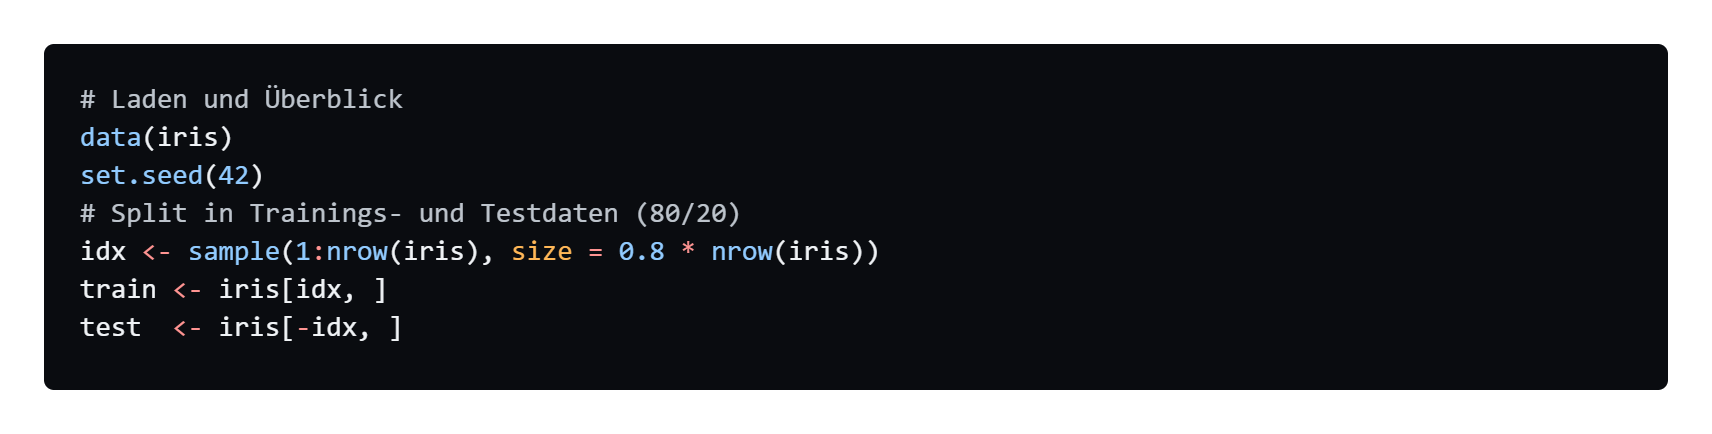
\includegraphics[scale=0.25]{iris_1_R.png}\\

In Python kam folgender Code zum Einsatz:\\
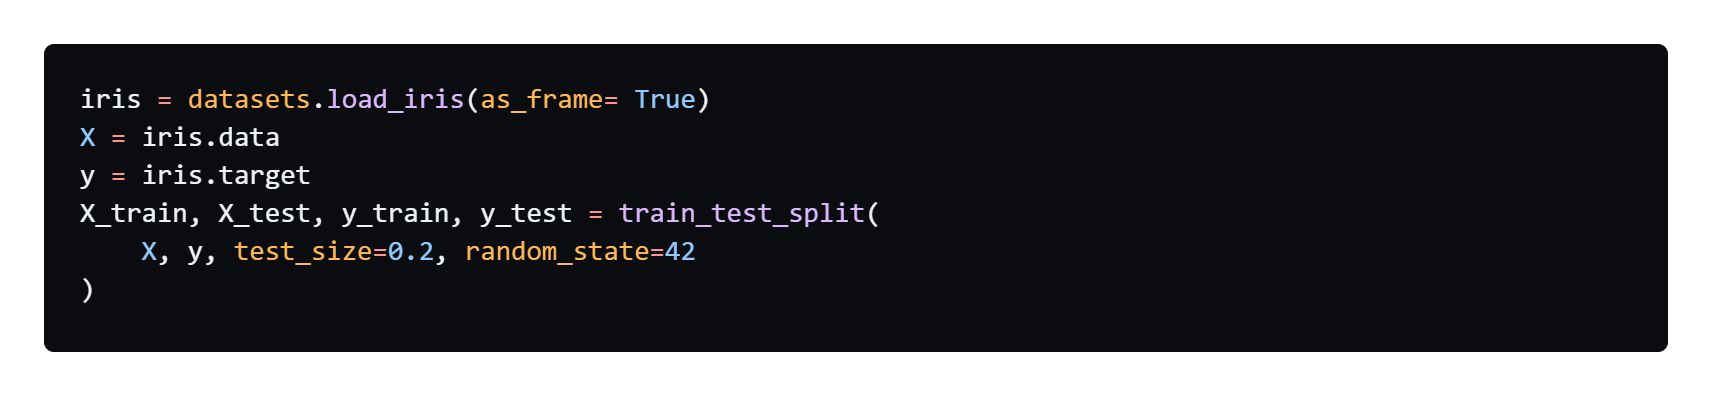
\includegraphics[scale= 0.25]{iris_1_py.png}\\
In Orange wurde der Workflow mit den Modulen File $\to$ Data Sampler (80/20) $\to$ Random Forest $\to$ Test \& Score realisiert. In RapidMiner wurde ein äquivalenter Prozess mit den Schritten Read CSV $\to$ Split Data $\to$ Random Forest $\to$ Apply Model $\to$ Performance umgesetzt.

Zur Evaluation wurden Metriken wie Accuracy, Precision, Recall, F1-Score und die Confusion Matrix herangezogen.\\
In R:\\
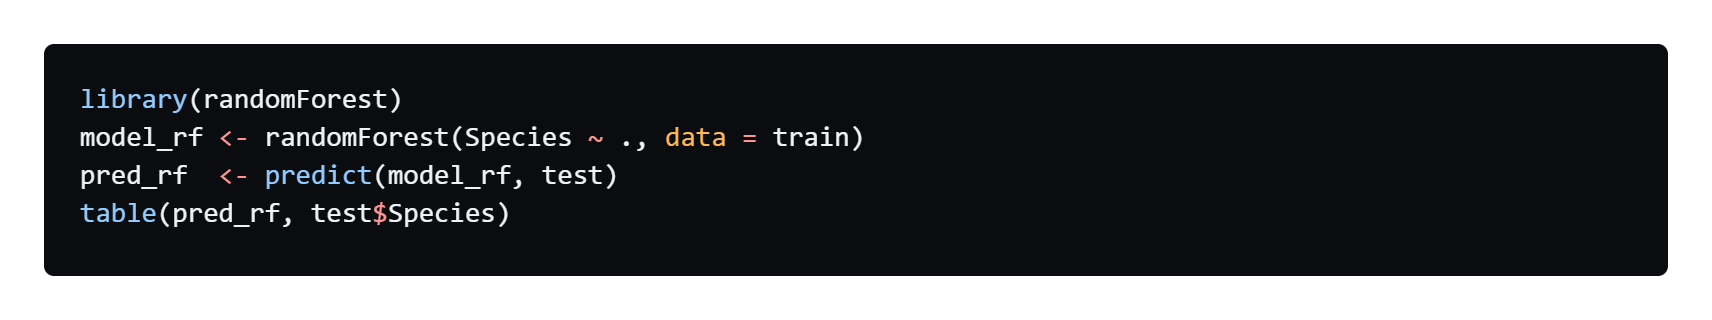
\includegraphics[scale=0.25]{iris_2_R.png}\\
In Python:\\
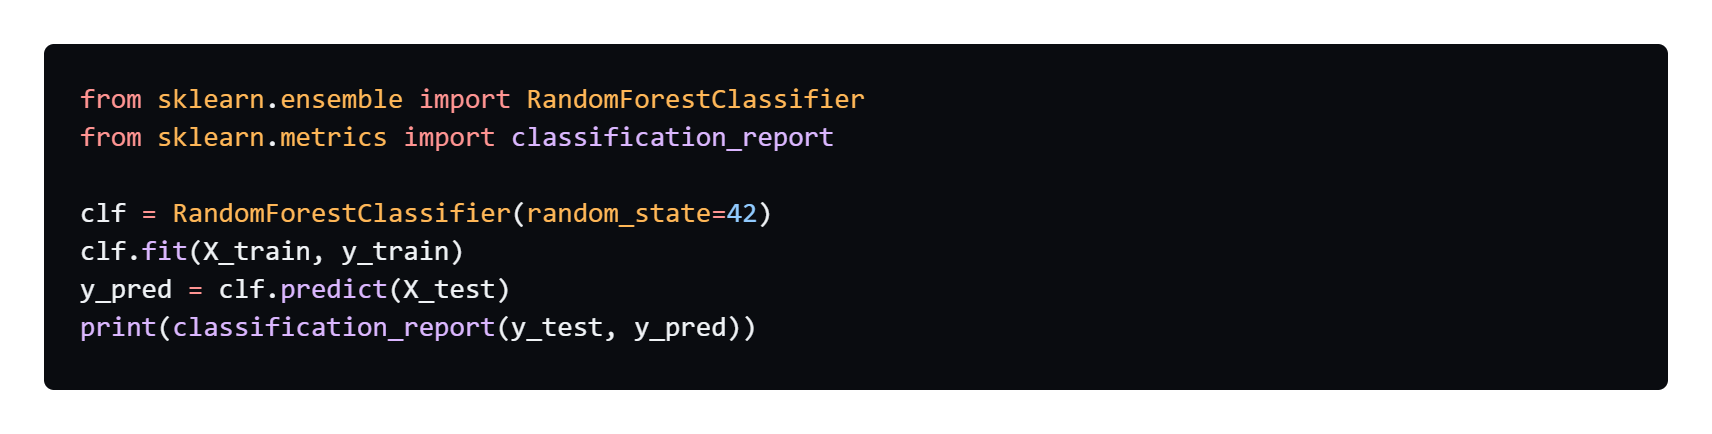
\includegraphics[scale=0.25]{iris_2_py.png}\\
\newline
\textbf{Ergebnisse (Python/R):}\\
R:
\begin{table}[!h]
\begin{tabular}{lllll}
pred\_rf   & setosa & versicolor & virginica &  \\
setosa     & 9      & 0          & 0         &  \\
versicolor & 0      & 10         & 1         &  \\
virginica  & 0      & 1          & 9         & 
\end{tabular}
\end{table}

Python:
\begin{table}[!h]
\begin{tabular}{lllll}
precision    & recall & f1-score & support &    \\
virginica    & 1.00   & 1.00     & 1.00    & 10 \\
setosa       & 1.00   & 1.00     & 1.00    & 9  \\
versicolor   & 1.00   & 1.00     & 1.00    & 11 \\
accuracy     & 1.00   & 30       &         &    \\
macro avg    & 1.00   & 1.00     & 1.00    & 30 \\
weighted avg & 1.00   & 1.00     & 1.00    & 30
\end{tabular}
\end{table}
\newline
\textbf{Interpretation:} Das Modell zeigt eine sehr gute Trennschärfe, insbesondere zwischen \textit{setosa} und den anderen beiden Arten.


\section*{Aufgabe 2: Algorithmusvergleich (Decision Tree, Naive Bayes, SVM)}

\textbf{Ziel:} Vergleich der Klassifikationsleistung dreier Algorithmen auf demselben Datensatz und Splits.\

\textbf{Vorgehen:} Als Datenbasis diente erneut der Iris-Datensatz. Die Daten wurden wie in Aufgabe 1 aufgeteilt. Es wurden drei Modelle trainiert:

\textbf{Decision Tree:} R: \lstinline|rpart()|, Python: \lstinline|DecisionTreeClassifier()|, Orange: Decision Tree-Widget, RapidMiner: Decision Tree $\to$ Apply Model.

\textbf{Naive Bayes:} R: \lstinline|e1071::naiveBayes()|, Python: \lstinline|GaussianNB()|, Orange: Naive Bayes-Widget, RapidMiner: Naive Bayes $\to$ Apply Model.

\textbf{SVM:} R: \lstinline|e1071::svm()|, Python: \lstinline|SVC()|, Orange: SVM-Widget, RapidMiner: SVM $\to$ Apply Model.

Die Modelle wurden mit Accuracy, Precision, Recall, F1 und ROC-AUC (für binäre und multiklassige Klassifikation) verglichen.\\
Hier als Beispiel der Decision Tree der durch das Python script erzeugt wurde:\\
\begin{figure}[htbp]
  \centering
  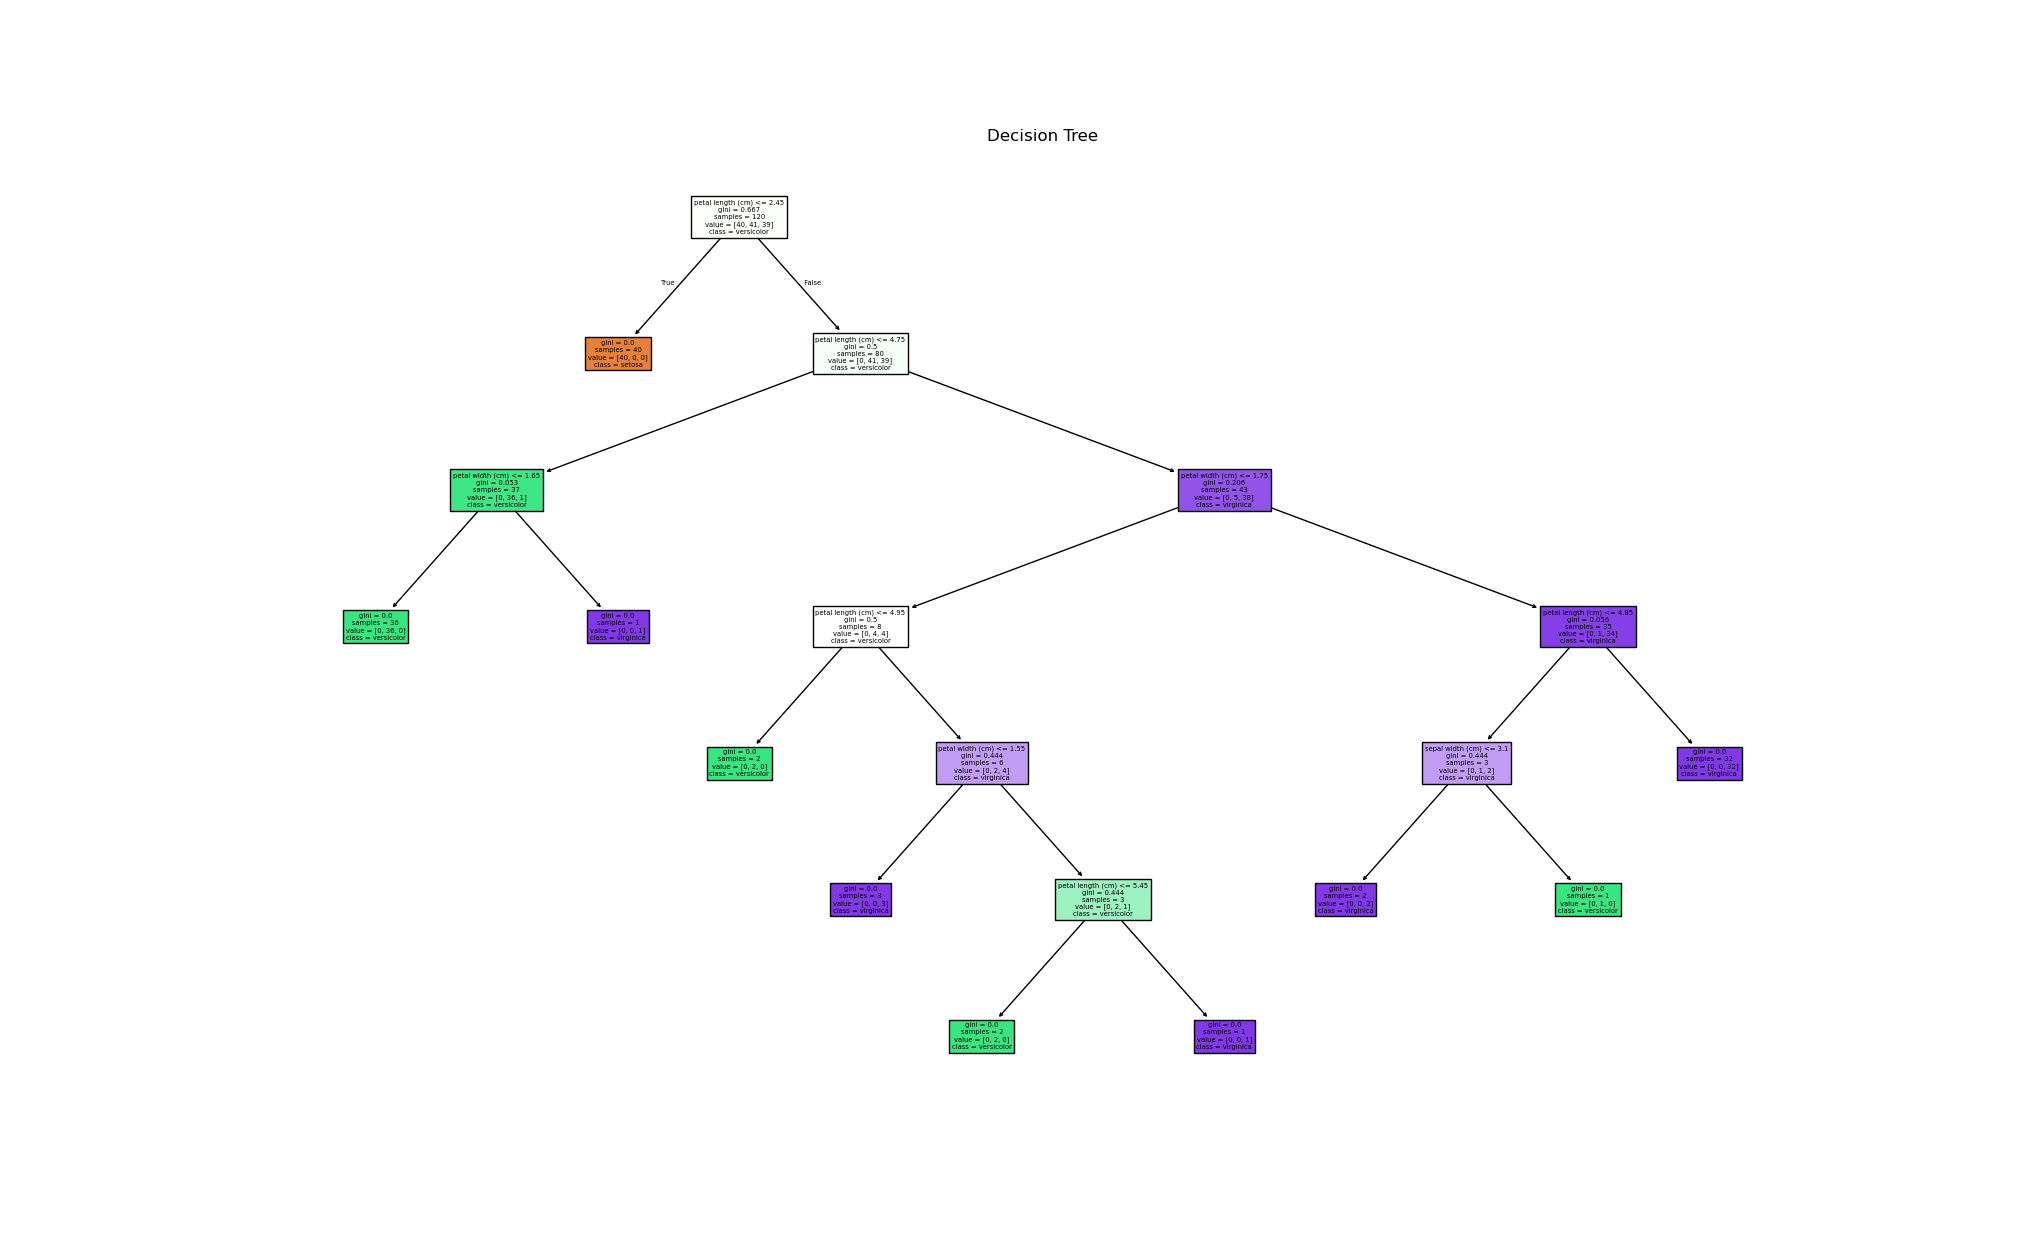
\includegraphics[scale=0.29]{Decision_tree.png}
  \caption{Auf meinem Discord ist das ganze auch noch mal in Hochauflösender \href{https://github.com/7hands/Angewandte-Modellierung-25-Colmant/blob/ec393fbadefd2cd1f55424f5d22f02f7f0c764c9/Assignment10/Tex/Decision_tree_py.svg}{link}}
\end{figure}



\textbf{Interpretation:} Alle Confusion Matrizen sind genau so wie die obigen aus Aufgabe 1 heißt alle classen wurden richtig zugeordnet.
\newpage


\section*{Aufgabe 3: Unüberwachtes Clustering (Rotwein‑Daten) mit Python}

Das Ziel dieser Aufgabe ist es, im „Wine“‑Datensatz mithilfe zweier Clustering‑Verfahren, nämlich K‑Means und hierarchischem Clustering, verborgene Gruppen in den Daten zu identifizieren. Dabei konzentrieren wir uns auf die chemischen Kenngrößen der Weine und untersuchen, ob sich anhand statistischer Kriterien sinnvolle Cluster bilden lassen.


Für das K‑Means‑Clustering wird das Modell mit \texttt{KMeans(n\_clusters=3, random\_state=42)} trainiert; parallel dazu wird ein hierarchisches Modell mit Ward‑Linkage über \texttt{AgglomerativeClustering(n\_clusters=3, linkage='ward')} erstellt und sein Dendrogramm mit \texttt{scipy.cluster.hierarchy.dendrogram} visualisiert. Die resultierenden Cluster werden anschließend durch die Berechnung der mittleren Feature‑Werte pro Gruppe charakterisiert und im zweidimensionalen Raum der ersten beiden Hauptkomponenten (PCA) farblich dargestellt.

Daraus ergibt sich dieses Hirachische Cluster:\\
\includegraphics*[scale=0.6]{Hirac_clustering.png}\\
und diese PCA:\\
\includegraphics*[scale=0.6]{PCA_py.png}
Als Ergebnis zeigt sich, dass drei Cluster die beste Kompromisslösung zwischen Kompaktheit und Trennschärfe liefern.

\newpage

\section*{Aufgabe 4: Google Trends Clustering}
Ich habe mir Trend daten zu 4 verschiednen themen rausgesucht und noch eine extra tabelle mit hilfe von den Wahlergebnissen der letzten buindestagwahl erstellt. Einmal Vergleiche ich Klima mit dem Fleischintresse und vergleiche dann noch ob die Geodaten von den Suchanfragen im zusammenhang zu den Wahlwerten der AFD haben.\\
Dann habe ich noch probiert den intressens umschwung von League of Legends auf Valorant einzufangen aber das hat so semi geklappt.\\
\includegraphics*[scale=0.6]{ValoLOLTime.png}\\
Wie man sieht sind die beiden spiele seit dem Valorant aus der Beta ist ungefähr auf dem selben intressen level, dass könnte daran liegen das viele Lol spieler auch valorant spieler sind und umgekehrt.\\
Jetzt zum interressanten teil:\\
\begin{table}[h!]
\begin{tabular}{llll}
Region                 & Value\_Klima & Value\_Schwein & Value\_Faschos \\
Berlin                 & 100          & 82             & 15.2           \\
Hessen                 & 98           & 71             & 17.7           \\
Bremen                 & 84           & 61             & 15.2           \\
Brandenburg            & 82           & 86             & 34.4           \\
Rheinland-Pfalz        & 80           & 88             & 19.2           \\
Hamburg                & 80           & 72             & 11.0           \\
Bayern                 & 73           & 100            & 17.4           \\
Schleswig-Holstein     & 72           & 85             & 16.1           \\
Baden-Württemberg      & 72           & 87             & 19.4           \\
Sachsen                & 71           & 64             & 38.5           \\
Niedersachsen          & 69           & 81             & 17.6           \\
Nordrhein-Westfalen    & 67           & 79             & 16.4           \\
Saarland               & 66           & 74             & 21.6           \\
Thüringen              & 65           & 69             & 38.7           \\
Mecklenburg-Vorpommern & 64           & 64             & 37.0           \\
Sachsen-Anhalt         & 61           & 61             & 38.8          
\end{tabular}
\end{table}
ich habe die Suchterme Klima und Schweinebauch als gegenidee des Weltkonsums gegenübergestellt. Dazu habe ich die Wahlwerte der letzten Bundestagswahl für die AFD per Bundesland raus gesucht (Spalte Faschos in Porzent).\\
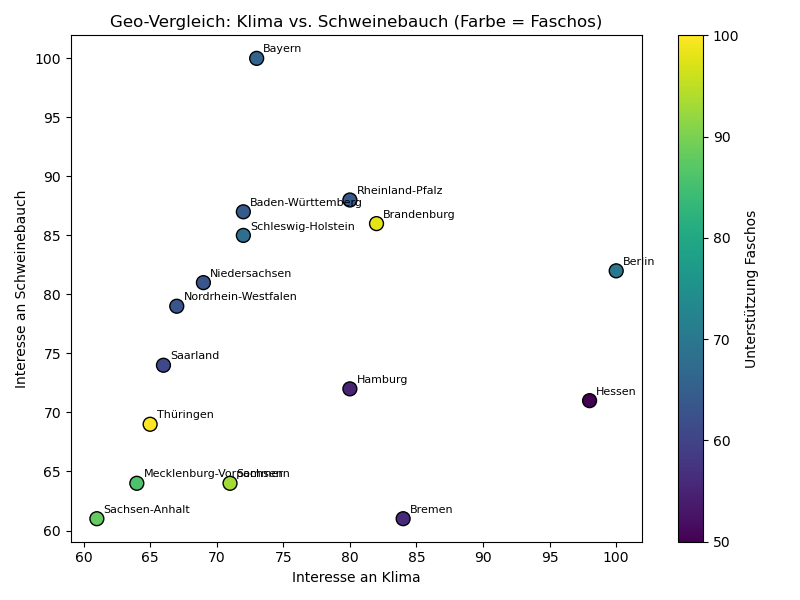
\includegraphics[scale=0.4]{KliSchwaFaschGEO.png}
\includegraphics*[scale=0.4]{PCA_KLI.png}\\

Wie man sehen kann sind viele der alten Ost und Westländer in je einer Gruppe. Zusätzlich entstehen noch zwei weiter gruppen die aus Hessen und Berlin, und die Aus Bremen und Hamburg. Die Berlin, Hessen Gruppe fällt auf durch starkes Klima interresse und swächere AFD Werte wärend die andere extra Gruppe wenig intresse an weder Klima noch Schweinefleisch hat aber auch eher schwache AFD Werte hat. In der ersten Graphik (links) sieht man auch das die Ost länder generell weniger diese beiden dinge gegoogled haben, vielleicht liegt das an erst späteren zugang zu weit verbreiteten Internet oder and einer generellen politischen unintresse.

\section*{\href{https://github.com/7hands/Angewandte-Modellierung-25-Colmant}{Github}}
Wie immer sind alle meine benutzten Dateien auf meinem Github zu finden. 
\end{document}
